\documentclass[journal,12pt,twocolumn]{IEEEtran}

\usepackage{setspace}
\usepackage{gensymb}


\singlespacing

\usepackage[cmex10]{amsmath}
%\usepackage{amsthm}
%\interdisplaylinepenalty=2500
%\savesymbol{iint}
%\usepackage{txfonts}
%\restoresymbol{TXF}{iint}
%\usepackage{wasysym}
\usepackage{amsthm}

\usepackage{mathrsfs}
\usepackage{txfonts}
\usepackage{stfloats}
\usepackage{bm}
\usepackage{cite}
\usepackage{cases}
\usepackage{subfig}

\usepackage{longtable}
\usepackage{multirow}

\usepackage{enumitem}
\usepackage{mathtools}
\usepackage{steinmetz}
\usepackage{tikz}
\usepackage{circuitikz}
\usepackage{verbatim}
\usepackage{tfrupee}
\usepackage[breaklinks=true]{hyperref}

\usepackage{tkz-euclide} %loads TikZ and tkz-base

\usetikzlibrary{calc,math}
\usepackage{listings}
    \usepackage{color}                                          
    \usepackage{array}                                          
    \usepackage{longtable}                                      
    \usepackage{calc}                                           
    \usepackage{multirow}                                       
    \usepackage{hhline}                                         
    \usepackage{ifthen}
    \usepackage{lscape}     
\usepackage{multicol}
\usepackage{chngcntr}

\DeclareMathOperator*{\Res}{Res}

\renewcommand\thesection{\arabic{section}}
\renewcommand\thesubsection{\thesection.\arabic{subsection}}
\renewcommand\thesubsubsection{\thesubsection.\arabic{subsubsection}}

\renewcommand\thesectiondis{\arabic{section}}
\renewcommand\thesubsectiondis{\thesectiondis.\arabic{subsection}}
\renewcommand\thesubsubsectiondis{\thesubsectiondis.\arabic{subsubsection}}

\hyphenation{op-tical net-works semi-conduc-tor}
\def\inputGnumericTable{}                                 %%

\lstset{
%language=C,
frame=single, 
breaklines=true,
columns=fullflexible
}

\begin{document}

\newtheorem{theorem}{Theorem}[section]
\newtheorem{problem}{Problem}
\newtheorem{proposition}{Proposition}[section]
\newtheorem{lemma}{Lemma}[section]
\newtheorem{corollary}[theorem]{Corollary}
\newtheorem{example}{Example}[section]
\newtheorem{definition}[problem]{Definition}

\newcommand{\BEQA}{\begin{eqnarray}}
\newcommand{\EEQA}{\end{eqnarray}}
\newcommand{\define}{\stackrel{\triangle}{=}}

\bibliographystyle{IEEEtran}

\providecommand{\mbf}{\mathbf}
\providecommand{\pr}[1]{\ensuremath{\Pr\left(#1\right)}}
\providecommand{\qfunc}[1]{\ensuremath{Q\left(#1\right)}}
\providecommand{\sbrak}[1]{\ensuremath{{}\left[#1\right]}}
\providecommand{\lsbrak}[1]{\ensuremath{{}\left[#1\right.}}
\providecommand{\rsbrak}[1]{\ensuremath{{}\left.#1\right]}}
\providecommand{\brak}[1]{\ensuremath{\left(#1\right)}}
\providecommand{\lbrak}[1]{\ensuremath{\left(#1\right.}}
\providecommand{\rbrak}[1]{\ensuremath{\left.#1\right)}}
\providecommand{\cbrak}[1]{\ensuremath{\left\{#1\right\}}}
\providecommand{\lcbrak}[1]{\ensuremath{\left\{#1\right.}}
\providecommand{\rcbrak}[1]{\ensuremath{\left.#1\right\}}}
\theoremstyle{remark}
\newtheorem{rem}{Remark}
\newcommand{\sgn}{\mathop{\mathrm{sgn}}}
\providecommand{\abs}[1]{\left\vert#1\right\vert}
\providecommand{\res}[1]{\Res\displaylimits_{#1}} 
\providecommand{\norm}[1]{\left\lVert#1\right\rVert}
%\providecommand{\norm}[1]{\lVert#1\rVert}
\providecommand{\mtx}[1]{\mathbf{#1}}
\providecommand{\mean}[1]{E\left[ #1 \right]}
\providecommand{\fourier}{\overset{\mathcal{F}}{ \rightleftharpoons}}
%\providecommand{\hilbert}{\overset{\mathcal{H}}{ \rightleftharpoons}}
\providecommand{\system}{\overset{\mathcal{H}}{ \longleftrightarrow}}
	%\newcommand{\solution}[2]{\textbf{Solution:}{#1}}
\newcommand{\solution}{\noindent \textbf{Solution: }}
\newcommand{\cosec}{\,\text{cosec}\,}
\providecommand{\dec}[2]{\ensuremath{\overset{#1}{\underset{#2}{\gtrless}}}}
\newcommand{\myvec}[1]{\ensuremath{\begin{pmatrix}#1\end{pmatrix}}}
\newcommand{\mydet}[1]{\ensuremath{\begin{vmatrix}#1\end{vmatrix}}}

\numberwithin{equation}{subsection}

\makeatletter
\@addtoreset{figure}{problem}
\makeatother

\let\StandardTheFigure\thefigure
\let\vec\mathbf

\renewcommand{\thefigure}{\theproblem}

\def\putbox#1#2#3{\makebox[0in][l]{\makebox[#1][l]{}\raisebox{\baselineskip}[0in][0in]{\raisebox{#2}[0in][0in]{#3}}}}
     \def\rightbox#1{\makebox[0in][r]{#1}}
     \def\centbox#1{\makebox[0in]{#1}}
     \def\topbox#1{\raisebox{-\baselineskip}[0in][0in]{#1}}
     \def\midbox#1{\raisebox{-0.5\baselineskip}[0in][0in]{#1}}
\vspace{3cm}

\title{Assignment 3}
\author{Surbhi Agarwal}

\maketitle

\newpage

%\tableofcontents

\bigskip

\renewcommand{\thefigure}{\theenumi}
\renewcommand{\thetable}{\theenumi}

\begin{abstract}
This document proves that a given equation represents two straight lines and finds the point of intersection and angle between them
\end{abstract}

Download all python codes from 
%
\begin{lstlisting}
https://github.com/surbhi0912/EE5609/
\end{lstlisting}
%
and latex-tikz codes from 
%
\begin{lstlisting}
https://github.com/surbhi0912/EE5609/
\end{lstlisting}
%
\section{Problem}
Prove that the following equations represent two straight lines; and also find their point of intersection and the angle between them
\begin{align}\nonumber
    x^2-5xy+4y^2+x+2y-2=0
\end{align}
\section{Solution}
\subsection{Proving that given equation represents two straight lines}
The general equation of second degree is given by
\begin{align}
    \label{eq:e1}ax^2+2bxy+cy^2+2dx+2ey+f=0\\
    \label{eq:e2}\implies \vec{x}^T\vec{V}\vec{x}+2\vec{u}^T\vec{x}+f=0
\end{align}
The given equation is
\begin{align}
    x^2-5xy+4y^2+x+2y-2=0
\end{align}
Comparing this to the standard equation \eqref{eq:e2}, we find
\begin{align}
    \vec{V} = \myvec{1 & \frac{-5}{2} \\ \frac{-5}{2} & 4}\\ \vec{u} = \myvec{\frac{1}{2} \\ 1}\\
    f = -2
\end{align}
\begin{align}\label{eq:e3}
    \implies\vec{x}^T\myvec{1 & \frac{-5}{2} \\ \frac{-5}{2} & 4}\vec{x} + 2\myvec{\frac{1}{2} & 1}\vec{x} -2 = 0
\end{align}
Equation \eqref{eq:e2} represents a pair of straight lines if
\begin{align}
    \label{eq:det}\mydet{\vec{V} & \vec{u}\\ \vec{u}^T & f}=0
\end{align}
\begin{align}
    \delta & = \mydet{1 & \dfrac{-5}{2} & \dfrac{1}{2} \\ \dfrac{-5}{2} & 4 & 1 \\ \dfrac{1}{2} & 1 & -2} \\ & = 0
\end{align}
Hence, proved that given equation represents two straight lines.
\subsection{Finding point of intersection between the straight lines}
\begin{align}
    \det V & = \mydet{1 & \frac{-5}{2}\nonumber\\ \frac{-5}{2} & 4}\\ & = \frac{-9}{4} < 0
\end{align}
Thus, the two straight lines intersect. Let the equation of the straight lines be given as
\begin{align}
    \label{eq:line1}\vec{n}_1^T\vec{x}=c_1 \\
    \label{eq:line2}\vec{n}_2^T\vec{x}=c_2
\end{align}
with their slopes as $\vec{m}_1$ and $\vec{m}_2$ respectively.

Then the equation of the pair of straight lines is
\begin{align}\label{eq:line1line2}
    (\vec{n}_1^T\vec{x}-c_1)(\vec{n}_2^T\vec{x}-c_2) = 0
\end{align}
Using \eqref{eq:e3} and \eqref{eq:line1line2},
\begin{align}
    (\vec{n}_1^T\vec{x}-c_1)(\vec{n}_2^T\vec{x}-c_2) = \vec{x}^T\myvec{1 & \frac{-5}{2} \\ \frac{-5}{2} & 4}\vec{x} + 2\myvec{\frac{1}{2} & 1}\vec{x} -2
\end{align}
Comparing both sides,
\begin{align}
    c_2\vec{n}_1+c_1\vec{n}_2 = -2\myvec{\frac{1}{2} \\ 1}\label{eq:c1c2}\\
    c_1c_2 = -2
\end{align}
Slopes of the lines are roots of the equation
\begin{align}
    cm^2+2bm+a=0 \label{eq:slope}\\
    \implies m_i = \frac{-b\pm \sqrt{-\mydet{\vec{V}}}}{c}\\
    \vec{n}_i = k_i\myvec{-m_i \\ 1}
\end{align}
Substituting \eqref{eq:e1} in \eqref{eq:slope},
\begin{align}
    4m^2-5m+1=0\\
    \implies m_i = \frac{\frac{5}{2}\pm \frac{3}{2}}{4} \\
    \implies m_1 = 1, m_2 = \frac{1}{4}
\end{align}
Therefore,
\begin{align}
    \vec{n}_1=k_1\myvec{-1 \\ 1}\\
    \vec{n}_2=k_2\myvec{\frac{-1}{4} \\ 1}
\end{align}
We know that
\begin{align}
	\label{n1n2}\vec{n}_1*\vec{n}_2 = \myvec{a\\2b\\c}\\
	k_1\myvec{-1 \\ 1}*k_2\myvec{\frac{-1}{4} \\ 1} = \myvec{1 \\ -5 \\ 4}\\
	\implies k_1k_2 = 4
\end{align}
Taking $k_1 = 1$, $k_2 = 4$, we get
\begin{align}
    \vec{n}_1 = \myvec{-1 \\ 1}\nonumber\\
    \vec{n}_2 = \myvec{-1 \\ 4}\label{eq:nvalues}
\end{align}
For verifying values of $\vec{n}_1$ and $\vec{n}_2$, we compute the convolution by representing $\vec{n}_1$ as Toeplitz matrix,
\begin{align}
    \vec{n}_1*\vec{n}_2=\myvec{-1 & 0 \\ 1 & -1 \\ 0 & 1}\myvec{-1 \\ 4} = \myvec{1 \\ -5 \\ 4}
\end{align}
Now, obtaining $c_1$ and $c_2$ using \eqref{eq:nvalues} and \eqref{eq:c1c2}
\begin{align}
    \myvec{\vec{n}_1 & \vec{n}_2}\myvec{c_2 \\ c_1} = -2\myvec{\frac{1}{2} \\ 1}\\
    \implies \myvec{-1 & -1 \\ 1 & 4}\myvec{c_2 \\ c_1} = \myvec{-1 \\ -2}
\end{align}
Row reducing the augmented matrix,
\begin{align}
    \myvec{-1 & -1 & -1 \\ 1 & 4 & -2} \xleftrightarrow{R_1 \leftarrow -R_1}\myvec{1 & 1 & 1 \\ 1 & 4 & -2}\xleftrightarrow{R_2\leftarrow R_2-R_1}\myvec{1 & 1 & 1 \\ 0 & 3 & -3}\\
    \xleftrightarrow{R_1\leftarrow R_1-R_2}\myvec{1 & 0 & 2 \\ 0 & 1 & -1}
\end{align}
\begin{align}
    \implies \myvec{1 & 0 \\ 0 & 1}\myvec{c_2 \\ c_1} = \myvec{2 \\ -1}\nonumber\\
    c_1 = -1\\
    c_2 = 2\label{eq:cvalues}
\end{align}
Thus, equation of lines can be written as
\begin{align}
    \myvec{-1 & 1}\vec{x} = -1\\
    \myvec{-1 & 4}\vec{x} = 2
\end{align}
Augmented matrix for these set of equations is
\begin{align}
    \myvec{-1 & 1 & -1 \\ -1 & 4 & 2}\xleftrightarrow{R_1\leftarrow -R_1}\myvec{1 & -1 & 1 \\ -1 & 4 & 2}\xleftrightarrow{R_2\leftarrow R_2+R_1}\myvec{1 & -1 & 1 \\ 0 & 3 & 3}\\
    \xleftrightarrow{R_2\leftarrow \frac{R_2}{3}}\myvec{1 & -1 & 1 \\ 0 & 1 & 1}\xleftrightarrow{R_1\leftarrow R_1+R_2}\myvec{1 & 0 & 2 \\ 0 & 1 & 1}
\end{align}
Thus, the point of intersection is $\vec{A} = \myvec{2 \\ 1}$

Using \eqref{eq:nvalues} and \eqref{eq:cvalues} in \eqref{eq:line1line2}, equation of the pair of straight lines is
\begin{align}
    (x-y-1)(x-4y+2) = 0
\end{align}
\renewcommand{\thefigure}{1}
\begin{figure}[h!]
    \centering
    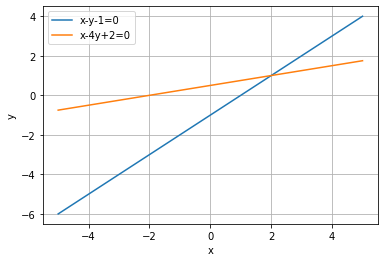
\includegraphics[width=\columnwidth]{assignment3.png}
    \caption{Intersection of lines}
    \label{fig:fig1}
\end{figure}
\subsection{Angle between lines}
Angle between pair of lines is,
\begin{align}\label{eq:cos}
    \theta = \cos^{-1}\left(\frac{\vec{n}_1^T\vec{n}_2}{\norm{\vec{n}_1}\norm{\vec{n}_2}}\right)
\end{align}
\begin{align}
    \vec{n}_1^T\vec{n}_2 = \myvec{-1 & 1}\myvec{-1 \\ 4} = 5 \label{eq:a2} 
\end{align}
\begin{align}
    \norm{\vec{n}_1}=\sqrt{(-1)^2+1^2}=\sqrt{2}\\
    \norm{\vec{n}_2}=\sqrt{(-1)^2+4^2}=\sqrt{17} \label{eq:}
\end{align}
Substituting these values \eqref{eq:cos}
\begin{align}
    \theta = 30.9\degree
\end{align}
Hence, angle between the given pair of straight lines is $30.9\degree$
\end{document}